\chapter{Условие}%
\label{cha:uslovie}

\begin{enumerate}
    \item 
        Назначить адреса подсетей:
        \begin{enumerate}
            \item 
                Подсеть 1: 192.168.x.0 /24
            \item 
                Подсеть 2: 192.168.x+1.0 /24
            \item 
                Подсеть 3: 192.168.x+2.0 /24
            \item 
                Подсеть 4: 192.168.x+3.0 /24
            \item 
                Подсеть 5 (В задаче 3): 192.168.x+10.0 /24
        \end{enumerate}

    \item 
        Настроить динамическую маршрутизацию в прилагаемом .pkt файле на стенде I через протокол RIPv2 так, чтобы пинг любым хостом или маршрутизатором любого другого хоста или маршрутизатора был успешным. Представить отдельным .pkt файлом.

    \item 
        Настроить динамическую маршрутизацию в сети в прилагаемом .pkt файле на стенде II через протокол OSPF так, чтобы пинг любым хостом или маршрутизатором любого другого хоста или маршрутизатора был успешным. Разделить при этом сеть на области OSPF в соответствии со схемой. Выполнить указания в лабораторной работе. Представить отдельным .pkt файлом.
\end{enumerate}

\chapter{Практическая часть}%
\label{cha:prakticheskaia_chast_}

\section{Назначение адресов подсетей}%

\begin{figure}[H]
    \centering
    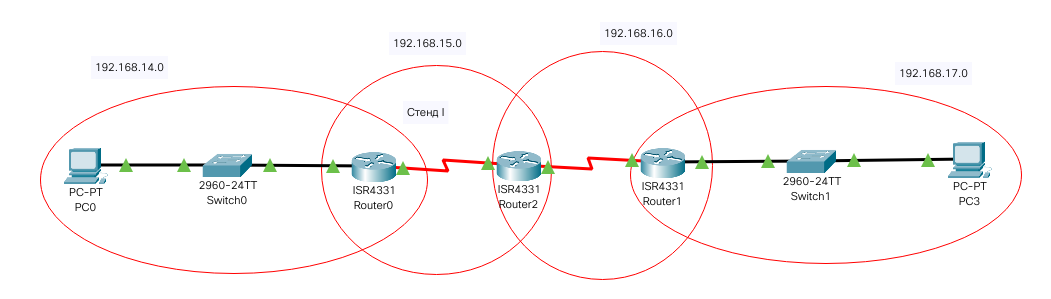
\includegraphics[width=0.8\linewidth]{images/scr01.png}
    \caption{Стенд \textnumero1}%
\end{figure}
\begin{figure}[H]
    \centering
    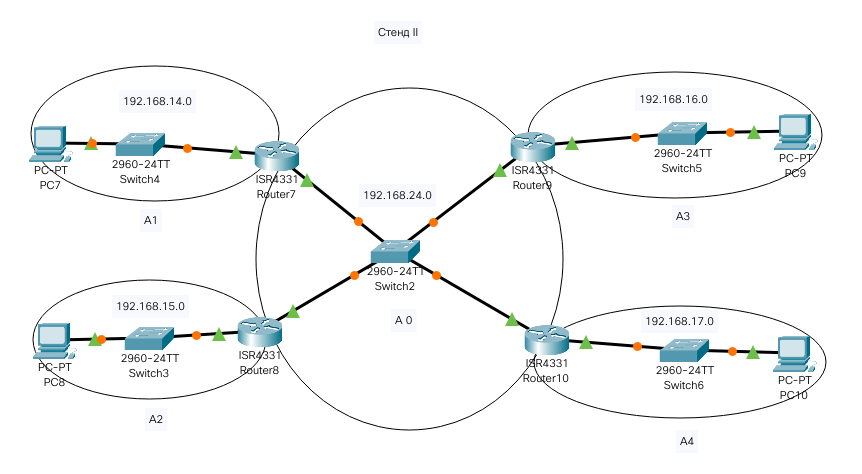
\includegraphics[width=0.8\linewidth]{images/scr02.png}
    \caption{Стенд \textnumero2}%
\end{figure}

\section{RIPv2}%
Команды для настройки RIPv2 представлены ниже. Для всех роутеров они аналогичны.
\begin{figure}[H]
    \centering
    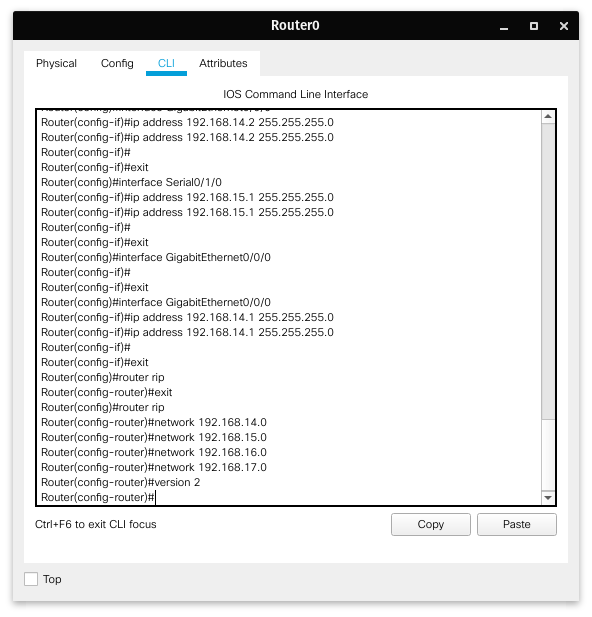
\includegraphics[width=0.8\linewidth]{images/scr03.png}
    \caption{}%
\end{figure}
Проверка соединения между PC0 и PC3:
\begin{figure}[H]
    \centering
    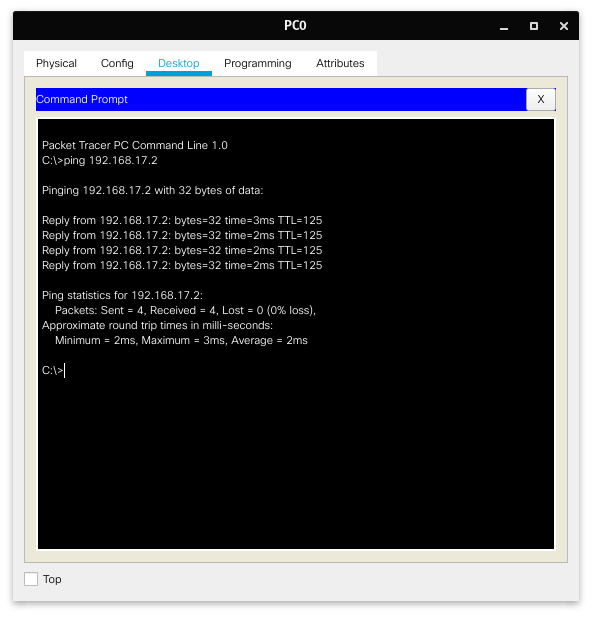
\includegraphics[width=0.8\linewidth]{images/scr04.png}
    \caption{}%
\end{figure}

\section{OSPF}%
Команды для настройки всех роутеров второго стенда приведены ниже.
\begin{figure}[H]
    \centering
    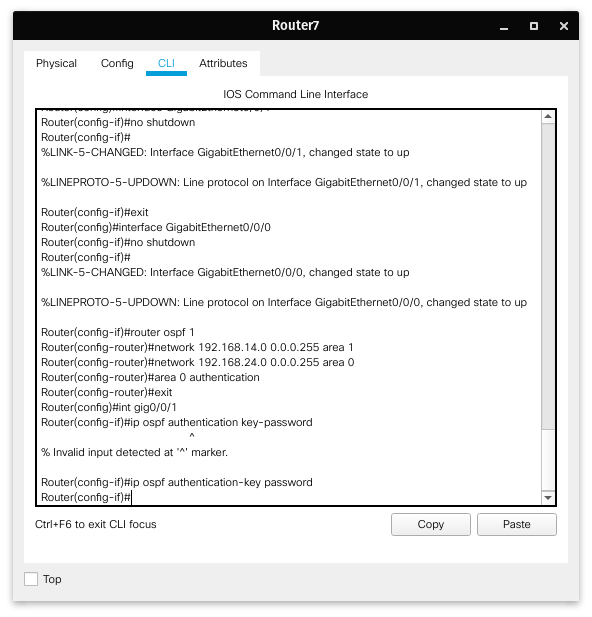
\includegraphics[width=0.8\linewidth]{images/scr05.png}
    \caption{}%
\end{figure}
\begin{figure}[H]
    \centering
    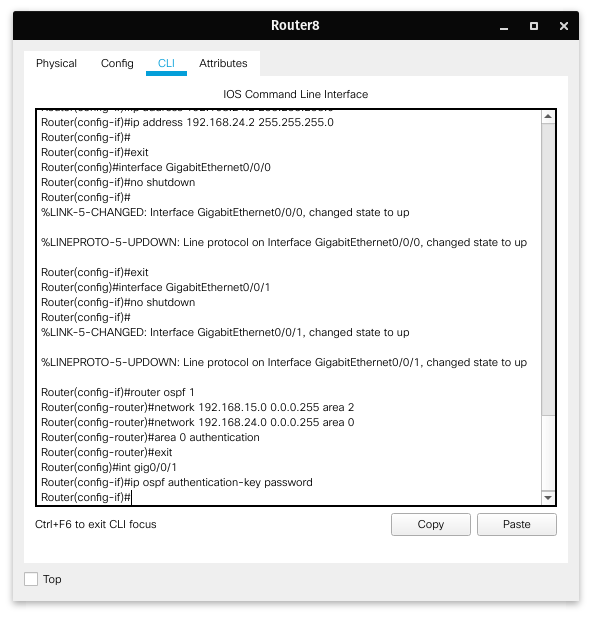
\includegraphics[width=0.8\linewidth]{images/scr06.png}
    \caption{}%
\end{figure}
\begin{figure}[H]
    \centering
    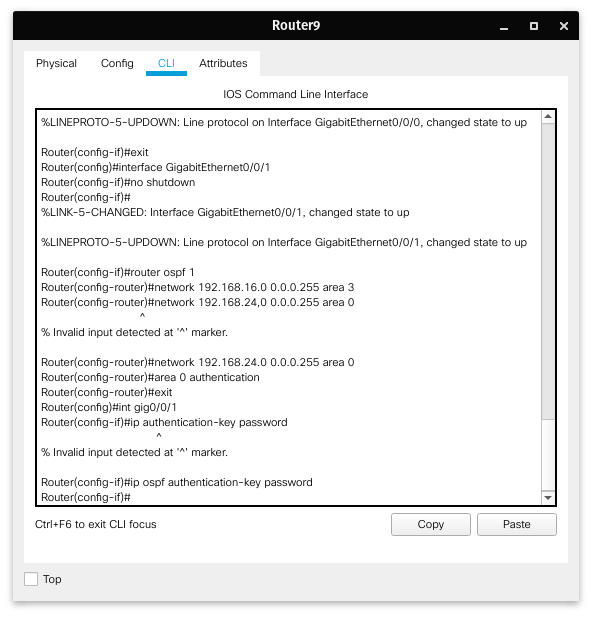
\includegraphics[width=0.8\linewidth]{images/scr07.png}
    \caption{}%
\end{figure}
\begin{figure}[H]
    \centering
    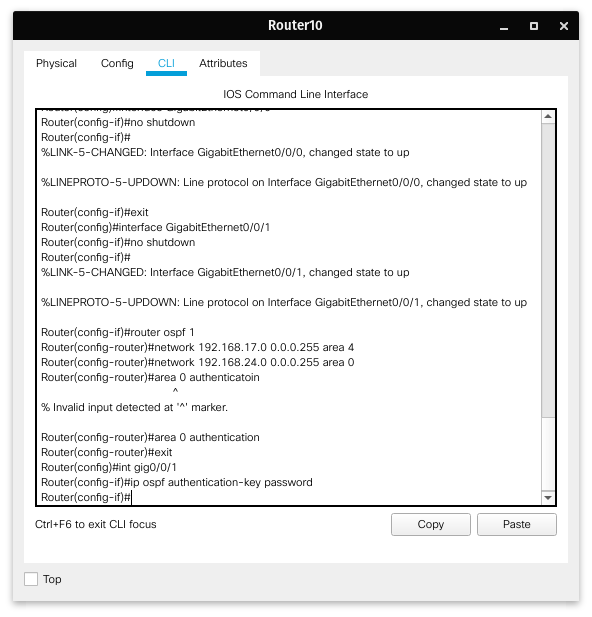
\includegraphics[width=0.8\linewidth]{images/scr08.png}
    \caption{}%
\end{figure}
Проверка соединения между PC9 и PC10:
\begin{figure}[H]
    \centering
    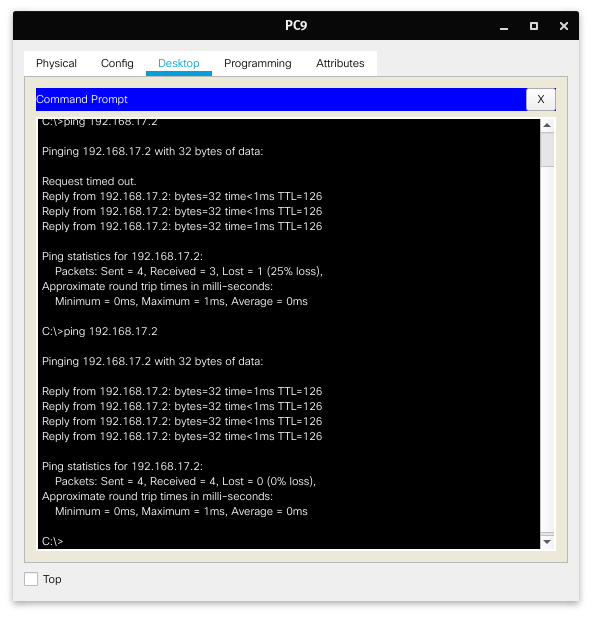
\includegraphics[width=0.8\linewidth]{images/scr9.png}
    \caption{}%
\end{figure}
